\documentclass[12pt]{article}

\usepackage{bbm}
\usepackage{fancyhdr}
\usepackage{titling}
\usepackage{enumitem}
\usepackage{amsmath}
\usepackage{dsfont}
\usepackage{amsfonts}
\usepackage{amssymb}
\usepackage{amsthm}
\usepackage{geometry}
\usepackage{tikz}
\usepackage{algorithm}
\usepackage{algpseudocode}
\geometry{verbose,tmargin=1in,bmargin=1in,lmargin=1in,rmargin=1in}
\renewcommand{\vec}[1]{\mathbf{#1}}
\newcommand{\dec}{\text{dec}}
\newcommand{\divi}{\mathbin{\textnormal{div}}}
\title{Homework 1}
\author{Satvik Prasad}
\date{}
\newtheorem{lemma}{Lemma}[section]
\fancypagestyle{plain}{%
  \fancyhf{}
  \fancyhead[L]{\theauthor}
  \fancyhead[R]{\thedate}
}
\pagestyle{plain}
\makeatletter
\def\@maketitle{%
  \newpage
  \null
  \vskip 1em%
  \begin{center}%
    \let \footnote \thanks
    {\LARGE \@title \par}%
    \vskip 1em%
  \end{center}%
  \par
\vskip 1em}
\makeatother
\usepackage{cmbright}

\newcommand{\mat}[1]{\mathbf{#1}}

% ---------- Probability theory ----------
% Core operators (optional argument-free; use as \E{X}, \Var{X}, \Cov{X}{Y})
\DeclareMathOperator{\EOp}{\mathbb{E}}
\DeclareMathOperator{\VarOp}{Var}
\DeclareMathOperator{\CovOp}{Cov}
\DeclareMathOperator{\CorrOp}{Corr}

\renewcommand{\P}[1]{\mathbb{P}\left(#1\right)}        % \P{A}
\newcommand{\E}[1]{\EOp\left[#1\right]}                % \E{X}
\newcommand{\Var}[1]{\VarOp\left(#1\right)}            % \Var{X}
\newcommand{\Cov}[2]{\CovOp\left(#1,\,#2\right)}       % \Cov{X}{Y}
\newcommand{\Corr}[2]{\CorrOp\left(#1,\,#2\right)}     % \Corr{X}{Y}
\newcommand{\SD}[1]{\operatorname{SD}\left(#1\right)}  % \SD{X}

% Subscripted versions, e.g. \Esub{\theta}{X}, \Psub{\theta}{A}
\newcommand{\Esub}[2]{\EOp_{#1}\left[#2\right]}
\newcommand{\Psub}[2]{\mathbb{P}_{#1}\left(#2\right)}

% Conditioning, indicators, independence
\newcommand{\given}{\,\middle|\,}                      % \E{X \given Y}
\newcommand{\ind}[1]{\mathbbm{1}\left\{#1\right\}}     % \ind{X > 0}
\newcommand{\indep}{\perp\!\!\!\perp}                  % X \indep Y
\newcommand{\iid}{\overset{\text{iid}}{\sim}}          % X_i \iid \Normal(0,1)

% Convergence
\newcommand{\convp}{\xrightarrow{\;p\;}}               % in probability
\newcommand{\convd}{\xrightarrow{\;d\;}}               % in distribution
\newcommand{\convas}{\xrightarrow{\text{a.s.}}}        % almost surely
\newcommand{\convLp}[1]{\xrightarrow{L^{#1}}}          % in L^p

% Probability spaces
\newcommand{\F}{\mathcal{F}}                           % sigma-algebra
\newcommand{\B}{\mathcal{B}}                           % Borel sigma-algebra
\newcommand{\pspace}{(\Omega, \F, \mathbb{P})}

% Common distributions
\newcommand{\Normal}{\mathcal{N}}
\newcommand{\Bern}{\operatorname{Bernoulli}}
\newcommand{\Bin}{\operatorname{Binomial}}
\newcommand{\Pois}{\operatorname{Poisson}}
\newcommand{\Unif}{\operatorname{Uniform}}
\newcommand{\Exp}{\operatorname{Exp}}
\newcommand{\Geom}{\operatorname{Geometric}}
\newcommand{\Gam}{\operatorname{Gamma}}
\newcommand{\Beta}{\operatorname{Beta}}

% Number sets
\newcommand{\R}{\mathbb{R}}
\newcommand{\N}{\mathbb{N}}
\newcommand{\Z}{\mathbb{Z}}

\begin{document}
\subsection{Green Circle}
\begin{enumerate}
  \item[2] Apply AM-GM to the sequence of numbers $1, 2, \ldots, n,$ yielding
    $$
    \dfrac{1 + 2+ \ldots + n}{n} > \sqrt[n]{n!},
    $$
    since $1 \neq 2 \neq 3 \neq \ldots \neq n,$
    or equivalently,
    $$
    \dfrac{n + 1}{2}> \sqrt[n]{n!} \Rightarrow n! <
    \left(\dfrac{n+1}{2}\right)^{n}
    $$a
    for all integers $n \geq 2.$ \qed

  \item[3] Fix $S = 2(ab + bc + ac).$ Then, by AM-GM we know
    $$
    S \geq 6\sqrt[3]{a^2 b^2 c^2} = 6{V^{2/3}},
    $$
    with equality when $ab = bc = ac,$ i.e., $a = b = c.$ Hence,
    $$
    V \leq (S/6)^{3/2},
    $$
    and when the prism is a cube, we have
    $$
    V = \left(\dfrac{S}{6} \right)^{3/2}.
    $$ \qed

  \item[5] Notice that for any $a, b, c > 0,$ we have
    $$
    (a + b + c)(a^{-1} + b^{-1} + c^{-1}) = 3 + \dfrac{a}{b} +
    \dfrac{b}{a} + \dfrac{a}{c} + \dfrac{c}{a} + \dfrac{b}{c} + \dfrac{b}{c}.
    $$
    By AM-GM, $a/b + b/a \geq 2,$ meaning the above is $\geq 3 + 3(2) = 9.$

    Thus, we know that
    $$
    [(a +b) + (b + c) + (c +a)]\left(\dfrac{1}{a + b} + \dfrac{1}{b +
    c} + \dfrac{1}{c + a}\right) \geq 9.
    $$
    Our left hand side reduces to
    $$
    (a  + b + c)\left(
      \dfrac{1}{a + b}  + \dfrac{1}{b  + c} + \dfrac{1}{c + a}
    \right) \geq \dfrac{9}{2}.
    $$
    Distributing, we get
    $$
    3 + \dfrac{c}{a + b} + \dfrac{a}{b+c} + \dfrac{b}{c + a} \geq 9/2
    \Rightarrow \dfrac{a}{b + c} + \dfrac{b}{ c + a} + \dfrac{c}{a + b} \geq 3/2
    $$
    as required. \qed

    If $a, b, c$ are sides of a triangle, we have $$
    a \leq b + c, \ b \leq a + c, \ c \leq a + b.
    $$

    Thus, we get
    $$
    b + c, a + b, a + c \geq (a + b+ c)/ 2,
    $$
    meaning
    $$
    T \leq 2( a+ b+ c)/(a+b+c) = 2
    $$
    as required. \qed
\end{enumerate}

\subsection{Blue Square}
\begin{enumerate}
  \item[6] For $a, b, c > 0$ we know that
    \begin{align*}
      a^4 + b^4 &\geq 2a^2b^2 \\
      b^4 + c^4 &\geq 2b^2c^2 \\
      c^4 + a^4 &\geq 2c^2a^2,
    \end{align*}
    meaning
    \begin{align*}
      a^4 + b^4 +c ^4 \geq a^2b^2 + b^2c^2 + c^2 a^2.
    \end{align*}
    Equivalently, we have
    $$
    a^4 + b^4  + c^4 \geq \dfrac{a^4 + b^4 + c^4 + a^2b^2 + b^2 c^2 +
    a^2 c^2}{2}.
    $$
    Then, applying AM-GM yields
    \begin{align*}
      a^4 + b^2 c^2 &\geq 2a^2bc \\
      b^4 + c^2 a^2 &\geq 2b^2ca \\
      c^4 + a^2 b^2 &\geq 2c^2ab,
    \end{align*}
    and hence
    $$
    a^4 + b^4 + c^4 \geq a^2bc + ab^2 c + abc^2 = abc( a +b + c)
    $$
    as required. \qed

  \item[7] Assume $a, b > 0.$ Consider $P(\sqrt{ab})^2.$ We RTP
    $P(\sqrt{ab})^2 \leq P(a)P(b).$ We have
    $$
    P(\sqrt{ab}) = \sum_{j = 0}^{d} \sqrt{c_j}a^{j/2} \cdot \sqrt{c_j}b^{j/2}.
    $$
    Apply Cauchy Schwartz to
    $$
    \{\sqrt{c_j} a^{j/2}\}_{j = 0}^{d},  \ \{\sqrt{c_j} b^{j/2}\}_{j = 0}^{d},
    $$
    yielding
    $$
    P(\sqrt{ab})^2 \leq \left (\sum_{j =0}^{d} c_j a^j\right) \left (
      \sum_{j = 0}^{d} c_j b^{j}
    \right) = P(a) P(b).
    $$
    Thus, rooting both sides (since both sides are non-negative), we get
    $$
    P(\sqrt{ab})  \leq \sqrt{P(a) P(b)}
    $$
    as required. \qed

  \item [8] Consider lines $\ell_i$ drawn from $P$ to each vertex of
    the polygon, and lines $t_i$ drawn from $P$ to the closest point
    along each side.
    \begin{center}
      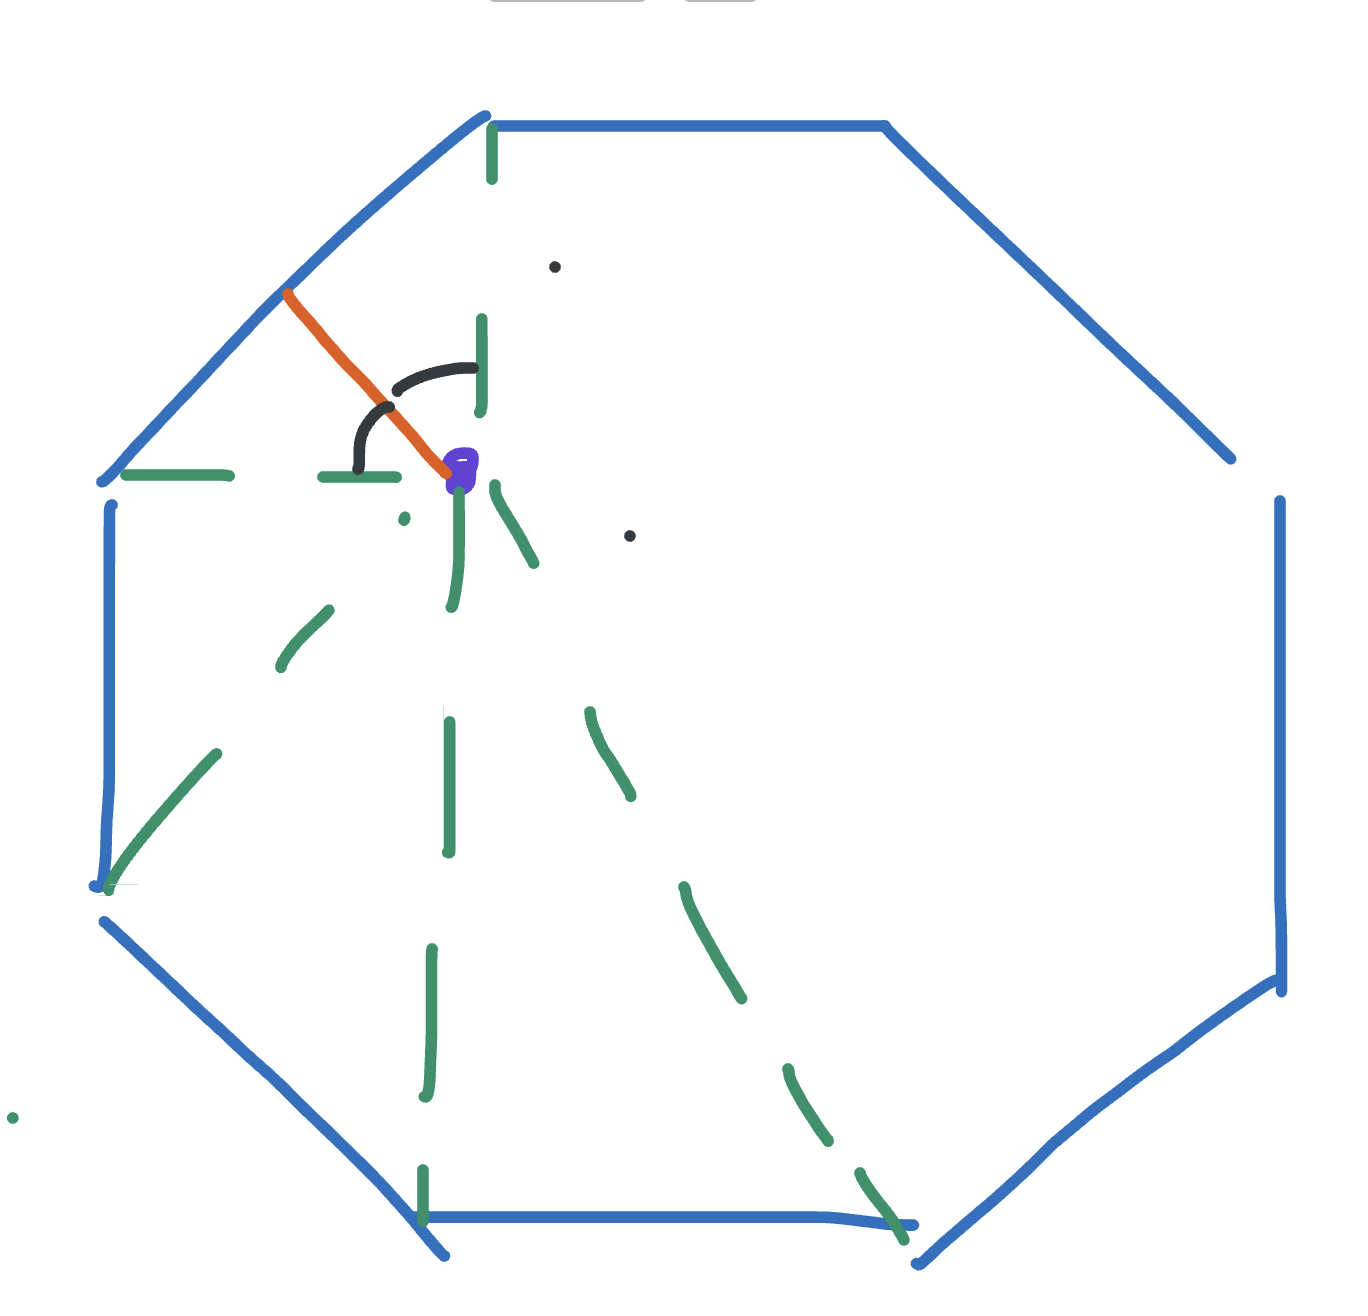
\includegraphics[width=0.3\linewidth]{math4802/img.png}
    \end{center}

    This creates $2n$ angles subtended between $t_i, \ell_i$ and
    $\ell_{i - 1}, t_i.$ Label the length of the opposite side of the
    triangle formed by $t_i, \ell_i$ as $a_i.$ Then,
    $$
    \tan\left(\dfrac{a_i}{|t_i|}\right) =
    \tan\left(\dfrac{a_i}{x_i}\right) = \angle t_i\ell_i,
    $$
    and similarly,
    $$
    \tan\left(\dfrac{1 - a_i}{|t_i|}\right) = \tan\left(\dfrac{1 -
    a_i}{x_i}\right) = \angle \ell_{i-1} t_i.
    $$
    Hence, summing over all such angles, we get
    $$
    2\pi = \sum_{i = 1}^{n} \tan\left(\dfrac{a_i}{x_i}\right) +
    \tan\left(\dfrac{1-a_i}{x_i}\right).
    $$
    Now, since $\tan x < x$ for all $x > 0,$ and either $a_i >0$ or
    $1 - a_i > 0,$ we get
    $$
    2\pi < \sum_{i = 1} ^{n} a_i/x_i + (1-a_i)/ x_i = \sum_{i =
    1}^{n} \dfrac{1}{x_i}
    $$
    as required. \qed
\end{enumerate}

\subsection{Black Diamond}
\begin{enumerate}
  \item[10] Rearranging, we get
    $$
    a^3 + b^3 + c^3 +3abc - a^2(b+c) - b^2(a+c) - c^2(a+b) \overset{?}{\geq }0.
    $$
    We can factor the left hand side as
    $$
    S = a(a-b)(a-c)  + b(b-a)(b-c) + c(c- a)(c-b).
    $$
    WLOG, assume $a \geq b \geq c.$ Then, we can write $S$ as
    $$
    S = a(a-b)(a-c) - b(a-b)(b-c) + c(a-c)(b-c).
    $$

    \begin{itemize}
      \item If $a = b,$ then we have $S = c(a-c)(b-c)$ which is
        composed of terms $\geq 0,$ and thus $S \geq 0.$

      \item Otherwise, factoring $a -b $ yields
        $$
        S = \underbrace{(a-b)}_{>0}[a(a-c) - b(b-c)] +
        \underbrace{c(a-c)(b-c)}_{\geq 0}>
        $$
        Since $a > b,$ we know $a(a-c) > b(b-c),$ and thus $S > 0.$
    \end{itemize}

    In either case, we get $S \geq 0,$ meaning
    $$
    a^3 + b^3 + c^3 + 3abc \geq a^2 (b+ c) + b^2 (c + a) + c^2 (a+b)
    $$
    as required. \qed

    For equality, we need $a= b$ and
    $$
    S= c(a-c)(b-c)= 0,
    $$
    since in the second case we never have equality.

    Hence, we have $a = b$ and $c = 0$, or $a = b= c.$ Thus, by
    symmetry in the general case, we need $a = b= c,$ or any two
    variables equal, and the third $0.$ \qed

  \item[11] Taking both sides to the power of $p,$ we get
    $$
    \sum_{i = 1}^{n}x_i^p \times \left(
      \sum_{i = 1}^{n} y_i^q
    \right)^{p/q} \overset{?}{\geq} \left(\sum_{i = 1}^{n} x_iy_i\right)^{p},
    $$
    or equivalently,
    $$
    \sum_{i = 1}^{n}x_i^p \left(
      \sum_{i = 1}^{n} y_i^q
    \right)^{1/q} \overset{?}{\geq} \left(\sum_{i = 1}^{n}
    x_i\dfrac{y_i}{\sum_{i = 1}^{n} y_i^q}\right)^{p}.
    $$
    To get weights that sum to $1$, we write
    $$
    \sum_{i = 1}^{n}x_i^p \left(
      \sum_{i = 1}^{n} y_i^q
    \right)^{1/q} \overset{?}{\geq} \left(\sum_{i = 1}^{n}
    \dfrac{x_i}{y_i^{q-1}}\dfrac{y_i^{q-1}}{\sum_{i = 1}^{n} y_i^q}\right)^{p}.
    $$

    Thus, we apply Jensen's to $x_i/y_i^{q-1}$ with weights
    $$y_i^{q}/\sum_{i = 1}^{n}y_i^q.$$ Since $x^p$ is convex, we have
    $$
    \sum_{i = 1}^{n} \dfrac{y_i^q}{\sum_{i = 1}^{n}y_i^q}
    \dfrac{x_i^p}{y_i^{qp - p}} \geq \left[\sum_{i = 1}^{n}
      \dfrac{y_i^q}{\sum_{i = 1}^{n}y_i^q} \left(
        \dfrac{x_i}{y_i^{q-1}}
    \right)\right]^{p}.
    $$
    Since $1/p + 1/q = 1, $ we know $p + q = qp,$ meaning $q + p - pq
    = 0,$ and hence the left hand side simplifies to
    $$
    \dfrac{1}{\sum_{i = 1}^{n}y_i^q}\sum_{i = 1}^{n} x_i^p \geq
    \left(\sum_{i = 1}^{n} x_i y_i\right)^p \cdot
    \left(\dfrac{1}{\sum_{i = 1}^{n} y_i^q}\right)^{p}.
    $$
    Rearranging, we have
    $$
    \left(\sum_{i = 1}^{n}y_i^q \right)^{p-1}  \sum_{i = 1}^{n} x_i^p
    \geq \left(\sum_{i = 1}^{n} x_i y_i\right)^p.
    $$
    Taking both sides to the power of $1/p,$ we have
    $$
    \left(
      \sum_{i = 1}^{n} x_i^p
    \right)^{1/p} \left(\sum_{i = 1}^{n}y_i^q\right)^{1-1/p} \geq
    \sum_{i = 1}^{n} x_i y_i.
    $$
    Since $1 - 1/p = 1/q,$ we finally have
    $$
    \left(
      \sum_{i = 1}^{n} x_i^p
    \right)^{1/p} \left(\sum_{i = 1}^{n}y_i^q\right)^{1/q} \geq
    \sum_{i = 1}^{n} x_i y_i
    $$
    as required. \qed
\end{enumerate}

\subsection{Reflection}
Had a plausible bound applying Jensen's to $x^p$ to weights $1/n,$
with a $n^{1/p + 1/q}$ term reducing to $1,$ but this was too loose
and resulted in RTP
$$
\sum_{i = 1}^{n} x_i \times \sum_{i = 1}^{n} y_i \geq n\sum_{i = 1}^{n} x_iy _i
$$
which is not true in the general case.

Required rearranging the statement and spotting the most natural
selection for the weights and terms for Jensen's, and proceding from there.

\end{document}
